\section{Chef}

\subsection{Tổng quan}
Chef là một framework cho việc tự động hóa hệ thống và cơ sở hạ tầng điện của toán đám mây. Chef được dùng để triển khai các máy chủ hoặc các ứng dụng tới bất kỳ đâu: từ máy chủ vật lý tới máy chủ ảo hay máy chủ trên hệ thống điện toán đám mây, mà không bao giờ phải bận tâm về kích thước của cơ sở hạ tầng. Chef-client dựa trên các định nghĩa trừu tượng (được gọi là cookbooks và recipes) được viết bằng Ruby và được quản lý như mã nguồn. Mỗi định nghĩa mô tả cách một phần cụ thể của cơ sở hạ tầng nên được xây dựng hoặc quản lý. Chef-client sau đó áp dụng những định nghĩa này cho các máy chủ và các ứng dụng, theo quy định, dẫn đến một cơ sở hạ tầng hoàn toàn tự động. Khi một node mới được đưa vào hệ thống, điều duy nhất mà chef-client cần biết là có những cookbooks và recipes nào cần phải được áp dụng.

\subsection{Kiến trúc hệ thống}

Sơ đồ dưới đây cho thấy mối quan hệ giữa các yếu tố khác nhau của Chef, bao gồm các nút, máy chủ, và các máy trạm. Những yếu tố này làm việc cùng nhau để cung cấp các chef-client các thông tin và hướng dẫn giúp nó thực hiện các công việc của mình.

\newpage
\clearpage

\begin{figure}[h!]
    \begin{center}
    \fbox{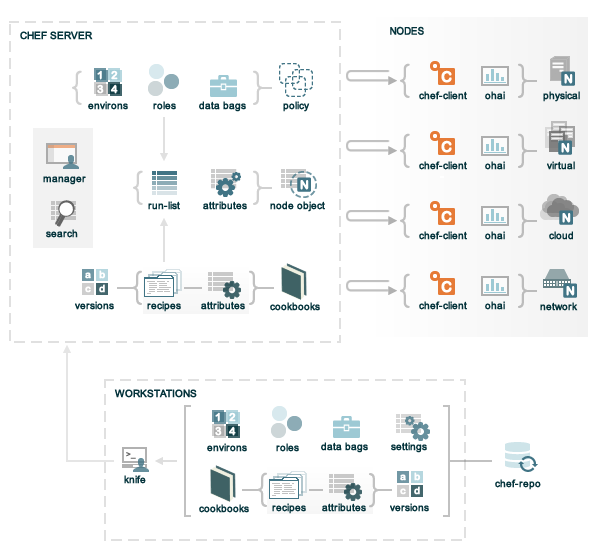
\includegraphics[width=\textwidth]{images/chef_overview.png}}
    \end{center}
    \caption{Mối quan hệ giữa các thành phần trong kiến trúc của Chef}
    \label{fig:chef_overview}
\end{figure}

Chef bao gồm ba yếu tố chính : một máy chủ trung tâm, một hay nhiều các nút, và ít nhất một máy trạm.

\begin{itemize}
\item Chef-server là máy chủ trung tâm. Nó phải luôn online để đảm bảo các chef-client có thể lấy được các cookbook và recipes để áp dụng.
\item Các máy trạm là nơi mà từ đó các cookbook và recipes được viết ra, các chính sách được định nghĩa. Dữ liệu ở đây được đồng bộ với chef-repo và cuối cùng tải lên server
\item Mỗi nút trong hệ thống đều có một chef-client quản lý. Chef-client có nhiệm vụ tự động hóa các công việc mà mỗi nút được yêu cầu.
\end{itemize}

Cookbook là một yếu tố rất quan trọng và có thể coi là một thành phần riêng biệt (cùng với máy chủ, máy trạm và các nút). Nhìn chung, cookbook được viết ra và quản lý bởi các máy trạm, sau đó được chuyển lên server; từ server chúng được đẩy xuống các nút bằng chef-client trong mỗi lần chef-client thực thi.

\subsection{Các thành phần chính}
Phần dưới đây sẽ cho chúng ta biết chi tiết hơn về các thành phần đã kể trên

\subsubsection{Các nút}


Một nút trong hệ thống của Chef có thể là một máy chủ vật lý, máy chủ ảo hoặc là một máy chủ trên mây, hoặc một thiết bị mạng. Chúng được cấu hình và duy trì bởi chef-client.

Một nút dựa trên đám mây thường được lưu trữ trong một số dịch vụ dựa trên điện toán đám mây, chẳng hạn như Amazon Virtual Private Cloud, OpenStack, Rackspace, Google Compute Engine, Linode, hoặc Windows Azure. Knife là công cụ của người quản trị hệ thống\footnote{Trong kiến trúc của chef thì knife có nghĩa là người quản trị hệ thống}, nó đã hỗ trợ sẵn các dịch vụ này. Knife có thể sử dụng các plugin để tạo ra các máy chủ trên hệ thống đám mây. Sau khi máy chủ đó được tạo ra, chef-client có thể được sử dụng để triển khai, cấu hình và duy trì những máy chủ này.

Một nút vật lý thường là một máy chủ hoặc một máy ảo, nhưng nó có thể là bất kỳ thiết bị gắn liền với hệ thống có khả năng gửi, nhận, và chuyển tiếp thông tin trên một kênh giao tiếp. Nói cách khác, một nút vật lý là bất kỳ thiết bị hoạt động nào gắn liền với hệ thống mà có thể chạy chef-client và cũng cho phép chef-client giao tiếp với máy chủ.

Các nút ảo thường mà các máy chủ ảo được tạo ra nhờ các phần mềm ảo hóa, cho dù vậy chúng có tính chất tương đương một nút vật lý.

Một nút mạng thường là các thiết bị mạng như swicth, router, VLAN hay những thứ tương tự mà có thể quản lý bằng chef-client.

Các thành phần quan trọng của nút bao gồm:

\textbf{Chef-client}

Chef-client là một agent chạy cục bộ trên tất cả các nút đã được đăng kí với máy chủ. Khi chef-client chạy, nó sẽ thực hiện tất cả các bước được yêu cầu để đưa nút vào trạng thái mong muốn. Những việc này bao gồm:

\begin{itemize}
\item Đăng ký và chứng thực các nút với máy chủ
\item Xây dựng các đối tượng nút
\item Đồng bộ hóa các cookbook
\item Biên dịch các tập hợp tài nguyên bằng cách tải về cookbook cần thiết, bao gồm cả recipes, các thuộc tính, cùng tất cả phụ thuộc khác
\item Thực hiện các hành động thích hợp và cần thiết để cấu hình các nút
\item Tìm kiếm ngoại lệ và các thông báo, và xử lý mỗi khi có yêu cầu
\end{itemize}

Cặp khóa công khai RSA được sử dụng để xác thực các chef-client với máy chủ mỗi khi chef-client cần truy cập vào dữ liệu được lưu trữ trên máy chủ. Điều này ngăn cản bất kỳ nút nào truy cập dữ liệu mà nó không nên truy cập và đồng thời cặp khóa này đảm bảo rằng chỉ có các nút đã được đăng ký với máy chủ có thể quản lý được các tài nguyên.

\textbf{Ohai}

Ohai là một công cụ được sử dụng để phát hiện các thuộc tính trên một nút, sau đó cung cấp những thuộc tính này cho chef-client tại mỗi lần chạy. Ohai là thành phần bắt buộc phải có của chef-client và nhất thiết phải có mặt trong một nút. Các loại thuộc tính mà Ohai thu thập bao gồm:

\begin{itemize}
\item Thông tin chi tiết về nền tảng
\item Thông tin về mức sử dụng tài nguyên mạng
\item Thông tin về mức sử dụng bộ nhớ
\item Thông tin về mức sử dụng CPU
\item Các thông tin về nhân hệ điều hành
\item Tên của máy chủ
\item Tên miền đầy đủ của máy chủ
\item Chi tiết cấu hình khác
\end{itemize}

Những thuộc tính được thu thập bởi Ohai là các thuộc tính tự động, trong đó các thuộc tính được sử dụng bởi các chef-client để đảm bảo rằng những thuộc tính này vẫn không thay đổi sau khi các chef-client được thực hiện cấu hình các nút.

\newpage
\clearpage

\subsubsection{Máy trạm}


Một máy trạm là một máy tính được cấu hình để chạy Knife. Nó cũng dùng để đồng bộ hóa với các chef-repo, cũng tương tác với một máy chủ duy nhất. Vị trí của máy trạm là nơi mà từ đó người dùng sẽ làm hầu hết công việc của họ, bao gồm:

\begin{itemize}
\item Phát triển các cookbook và recipes (sử dụng ngôn ngữ lập trình Ruby)
\item Đồng bộ hóa với chef-repo sử dụng hệ thống quản lý mã nguồn (Git hoặc SVN)
\item Sử dụng Knife để tải lên cái item từ chef-repo lên server
\item Cấu hình các chính sách của tổ chức, bao gồm cả việc định nghĩa các vai trò (roles) và môi trường, đồng thời đảm bảo việc dữ liệu quan trọng đã được lưu lại trong data bags
\item Tương tác với các nút khi cần thiết, chẳng hạn thiết lập bootstrap cho một nút.
\end{itemize}

\subsubsection{Knife}


Knife là một công cụ dòng lệnh cung cấp một giao diện giữa các chef-repo cục bộ tại máy trạm và máy chủ. Knife giúp cho người dùng có thể quản lý những điều sau:

\begin{itemize}
\item Các nút
\item Cookbooks và recipes
\item Roles
\item Lưu trự dữ liệu JSON (data bags), bao gồm cả dữ liệu mã hóa
\item Các thiết lập môi trường
\item Cái tài nguyên của điện toán đám mây, bao gồm cả tài nguyên dự phòng
\item Cài đặt các chef-client trên máy trạm quản lý
\item Tìm kiếm các thông tin được index trên máy chủ
\end{itemize}

\subsubsection{Chef-Repo}


Chef-repo là nơi mà các đối tượng dữ liệu sau được lưu trữ:

\begin{itemize}
\item Cookbooks (bao gồm cả recipes, phiên bản, các thuộc tính, tài nguyên, nhà cung cấp, thư viện và các mẫu)
\item Roles
\item Databags
\item Các thông số về môi trường làm việc
\item Các file cấu hình (cho máy khách, máy trạm và máy chủ)
\end{itemize}

Chef-repo nằm trên một máy trạm và cần được đồng bộ hóa với hệ thống quản lý mã nguồn, chẳng hạn như git. Tất cả các dữ liệu trong chef-repo nên được đối xử như là mã nguồn.

Knife được sử dụng để upload dữ liệu từ chef-repo lên máy chủ. Sau khi tải lên, dữ liệu được các chef-client sử dụng để quản lý tất cả các nút đã được đăng kí, đồng thời đảm bảo tất cả những thứ như cookbooks, cái thống số môi trường, roles và các thiết lập khác được áp dụng cho nút đó một cách đứng đắn.

\newpage
\clearpage

\subsubsection{Máy chủ}


Các máy chủ hoạt động như một trung tâm chứa dữ liệu cấu hình. Các máy chủ lưu trữ các cookbooks, chính sách sẽ được áp dụng cho các nút, và các metadata được quản lý bởi chef-client. Các nút sử dụng chef-client để yêu cầu máy chủ các thông tin chi tiết về cấu hình, chẳng hạn như recipes, templates hay các tệp tin. chef-client thực hiện các công việc của mình trên từng nút mà không phải là trên máy chủ. Cách tiếp cận theo hướng phân phối mở rộng này khá tương ứng với mô hình của Puppet.

Hosted Enterprise Chef là một phiên bản máy chủ của Chef. Hosted Enterprise Chef được xây dựng dựa trên điện toán đám mây, có khả năng mở rộng và luôn sẵn sàng 24x7/365. Hosted Enterprise Chef có thể quản lý bất kì máy chủ nào mà không yêu cầu nó phải được thiết lập và quản lý từ phía sau tường lửa.

\subsubsection{Cookbooks}


Cookbook là đơn vị cơ bản của Chef trong việc cấu hình và phân phối các chính sách. Mỗi cookbook định nghĩa một kịch bản, chẳng hạn như tất cả mọi thứ cần thiết để cài đặt và cấu hình MySQL, và sau đó nó chứa tất cả các thành phần được yêu cầu để hỗ trợ kịch bản đó, bao gồm:

\begin{itemize}
\item Các giá trị của thuộc tính được thiết lập trên các nút
\item Định nghĩa sự cho phép tạo ra hoặc sử dụng lại tập hợp các tài nguyên
\item Các thư viện dùng để mở rộng chef-client hoặc cung cấp sự trợ giúp bằng mã nguồn Ruby
\item Recipes là cách thức xác định các tài nguyên cần thiết để quản lý và thứ tự của chúng khi áp dụng
\item Các mẫu
\item Các phiên bản
\item Các siêu dữ liệu về cách thức (bao gồm cả các gói phụ thuộc), hạn chế phiên bản, nền tảng hỗ trợ hay những gì tương tự.
\end{itemize}

Chef-client sử dụng ngôn ngữ Ruby như một ngôn ngữ tham chiếu để tạo ra cookbook và xác định recipes, với DSL mở rộng cho các tài nguyên cụ thể. Chef-client cung cấp một tập hợp lý các tài nguyên, đủ để hỗ trợ rất nhiều các kịch bản tự động hóa cơ sở hạ tầng phổ biến nhấ. Tuy nhiên, DSL này cũng có thể được mở rộng khi có thêm tài nguyên và khả năng được yêu cầu.

\newpage
\clearpage

\subsection{Cài đặt và sử dụng}

\subsubsection{Cách cài đặt Chef (server và client)}

Hiện tại Chef-Server chỉ hỗ trợ gói cài đặt cho RHEL và Ubuntu. Chef-Client hỗ trợ đa nền tảng hơn hơn và có script cài đặt đi kèm.

\textbf{• Cách cài đặt Chef trên RHEL}

Đối với Chef-Server:

\begin{lstlisting}[label={lst:chef_install_server_rhel},caption={Cách cài đặt chef-server trên RHEL},language=bash]
# Install chef-server
rpm -ivh https://opscode-omnibus-packages.s3.amazonaws.com/el/6/x86_64/chef-server-11.0.10-1.el6.x86_64.rpm
# Initial configuration for chef-server
chef-server-ctl reconfigure
\end{lstlisting}

Đối với Chef-Client:

\begin{lstlisting}[label={lst:chef_install_client_rhel},caption={Cách cài đặt chef-client trên RHEL},language=bash]
# Install chef-client
curl -L https://www.opscode.com/chef/install.sh | bash
\end{lstlisting}

\textbf{• Cách cài đặt Chef trên Ubuntu}

Đối với Chef-Server:

\begin{lstlisting}[label={lst:chef_install_server_ubuntu},caption={Cách cài đặt chef-server trên Ubuntu},language=bash]
# Download chef-server package
wget https://opscode-omnibus-packages.s3.amazonaws.com/ubuntu/12.04/x86_64/chef-server_11.0.10-1.ubuntu.12.04_amd64.deb
# Install chef-server package
sudo dpkg -i chef-server_11.0.10-1.ubuntu.12.04_amd64.deb
# Initial configuration for chef-server
sudo chef-server-ctl reconfigure
\end{lstlisting}

\newpage
\clearpage

Đối với Chef-Client:

\begin{lstlisting}[label={lst:chef_install_client_ubuntu},caption={Cách cài đặt chef-client trên Ubuntu},language=bash]
# Install chef-client
curl -L https://www.opscode.com/chef/install.sh | bash
\end{lstlisting}

\textbf{Chú ý}: Chef-Server cần mở cổng 443 để các Chef-Client có thể liên lạc được với nó.

\textbf{• Cách cài đặt Knife trên máy trạm}

Như đã nói trong kiến trúc của Chef, cần có một máy trạm chứa công cụ Knife và chef-repo để đưa các lệnh tới máy chủ và các nút.

Vì vậy chúng ta phải cài đặt chef-client trên máy trạm này, cài đặt công cụ knife và đồng bộ chef-repo.

\begin{lstlisting}[label={lst:chef_install_knife},caption={Cách cài đặt knife và chef-repo},language=bash]
# Install chef-client
curl -O -L http://www.opscode.com/chef/install.sh | bash

# Clone the Chef Repo skeleton directory to work in:
cd ~/Development
git clone https://github.com/opscode/chef-repo.git
\end{lstlisting}

\newpage
\clearpage

\subsubsection{Cách cấu hình cơ bản hệ thống Chef}

Các bước cấu hình của Chef phức tạp hơn so với Puppet khá nhiều, ở đây chúng ta chỉ giới thiệu một số bước cấu hình đơn giản. Chi tiết về các cấu hình còn lại có thể tham khảo trên trang tài liệu của dự án:

\url{http://docs.opscode.com}

\begin{lstlisting}[label={lst:chef_basic_config},caption={Các bước cấu hình hệ thống Chef},language=bash]
# Config knife
knife configure
...

# List chef-client (nodes)
knife client list

# Bootstrap first client server
knife bootstrap -u $USERNAME --sudo $FQDN_OF_CLIENT_SERVER
\end{lstlisting}

\newpage
\clearpage

\subsection*{Tóm lại}

Các nguyên tắc cơ bản quan trọng của Chef là chúng ta (những người sử dụng) là những người biết rõ nhất về những gì môi trường của bản thân, những gì cần làm, và làm thế nào để duy trì được nó. Chef-client được thiết kế để không phá vỡ những điều như vậy. Và chỉ có chúng ta cũng như đồng nghiệp của chúng ta mới hiểu rõ ràng các vấn đề về kĩ thuật cũng như phải làm gì để giải quyết chúng. Chỉ chúng ta mới có thể hiểu được các vấn đề về con người(trình độ kỹ năng, những kĩ năng kiểm soát, và các vấn đề nội bộ khác), những thứ mà duy nhất chỉ doanh nghiệp hay tổ chức của bạn biết được giải pháp.

Ý tưởng ở đây là bạn nắm rõ trong tay những gì sẽ xảy ra với hệ thống của bạn, và cách như thế nào để làm nó hoạt động hiệu quả. Tuy nhiên, một cá nhân rất khó có thể nắm bắt được mọi thứ về một vấn đề phức tạp, cũng như các bước để giải quyết chúng. Vấn đề cũng tương tự với những công cụ này. Chef hỗ trợ chúng ta quản lý các cơ sở hạ tầng. Chef có thể giúp giải quyết các vấn đề phức tạp. Chef có một cộng đồng rộng lớn, nơi mọi người có rất nhiều các kinh nghiệm trong việc giải quyết các vấn đề phức tạp và họ có thể cung cấp các kiến thức hay hỗ trợ chúng trong lĩnh vực mà tổ chức chúng ta chưa có kinh nghiệm. Cộng đồng cũng với Chef có thể giúp doanh nghiệp hay tổ chức của chúng ta giải quyết các vấn đề phức tạp.
